\appendix
\chapter*{付録}
\section{シミュレーションソース格納先}
本研究で使用したシミュレーションソースコードは以下のGitHub上のリポジトリに格納している. 適宜参照されたい.
\begin{itemize}
  \item \url{https://github.com/tsyu12345/Rikkyo-MasterPJ}
\end{itemize}
\section{特別研究レポート格納先}
本研究経過過程である特別研究1/2および3と研究内容提案書のレポートは以下のリンクから閲覧可能である. 適宜参照されたい.
\begin{itemize}
  \item \href{https://drive.google.com/open?id=1cAxzPoKxxjQKVu29GLQ0nsldmYBtgDEn&usp=drive_fs}{特別研究1 報告書}
  \item \href{https://drive.google.com/open?id=14rU8VHIF_2HHVoE2twPA_s9i6qF9QqlJ&usp=drive_fs}{特別研究2 報告書}
  \item \href{https://drive.google.com/open?id=1cJ8v32mS4TthynS6yP99nYb8Sv3YQPLZ&usp=drive_fs}{研究内容提案書}
  \item \href{https://drive.google.com/open?id=1cLeL2UJFi6_QtMtjGqVr22aTDtoGnCT5&usp=drive_fs}{特別研究3 報告書}
  \item \href{https://drive.google.com/open?id=14ub9oX1HVd4acJh_h1ov97LJCkNjIwnq&usp=drive_fs}{特別研究3 別冊資料}
\end{itemize}

\section{探索タスクマルチエージェントモデルの学習結果}
\subsection{横須賀市の場合}
\begin{figure}[H] 
  \centering 
  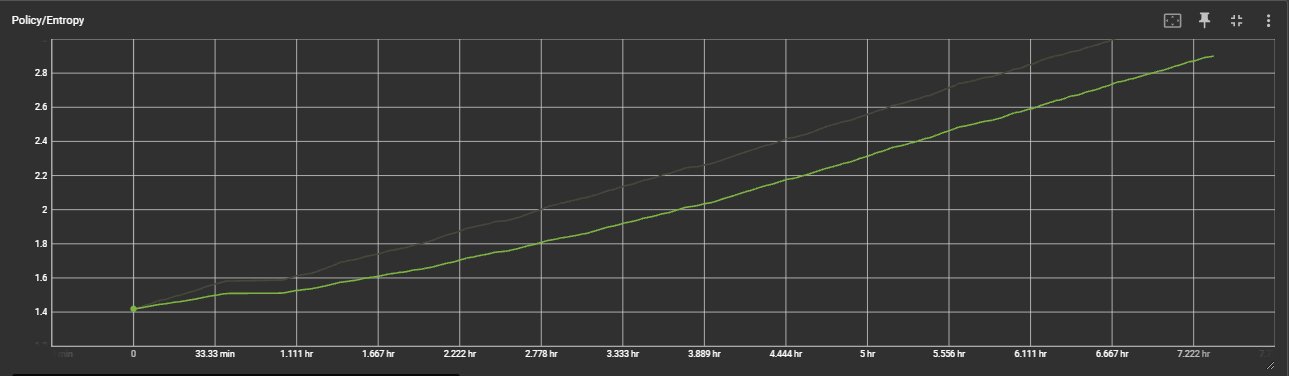
\includegraphics[width=0.8\textwidth]{Figures/App-YokosukaSearchEntropy.png}
  \caption{エントロピーの推移} 
  \label{fig:fig-01}
\end{figure}
\begin{figure}[H] 
  \centering 
  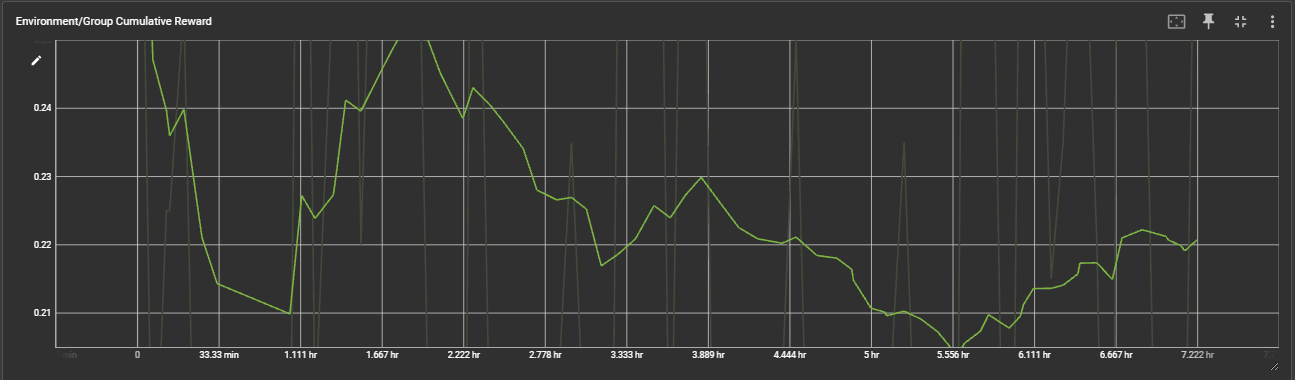
\includegraphics[width=0.8\textwidth]{Figures/App-YokosukaSearchGroupRward.png}
  \caption{グループ累積報酬の推移} 
  \label{fig:fig-01}
\end{figure}
\begin{figure}[H] 
  \centering 
  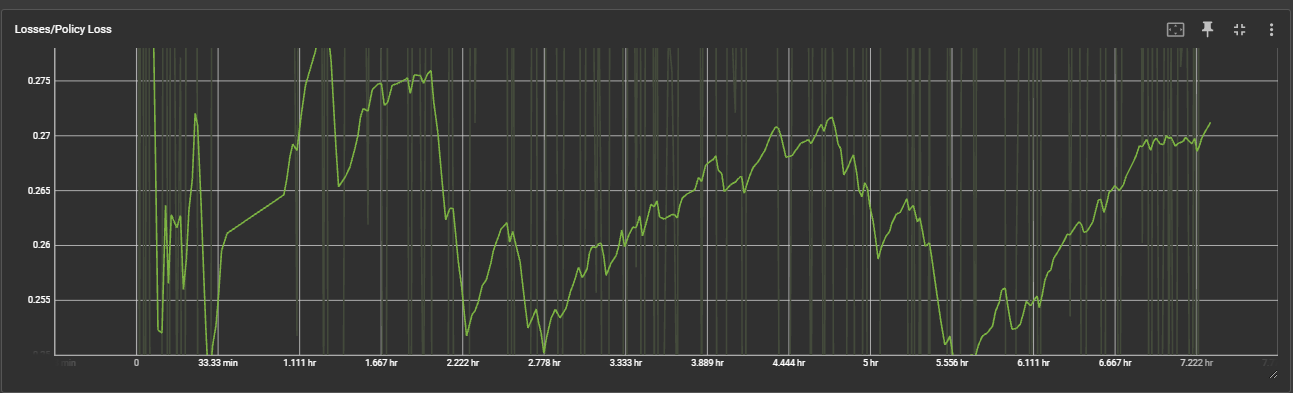
\includegraphics[width=0.8\textwidth]{Figures/YokosukaSearch-PolicyLoss.png}
  \caption{ポリシー関数の平均損失} 
  \label{fig:fig-01}
\end{figure}
\begin{figure}[H] 
  \centering 
  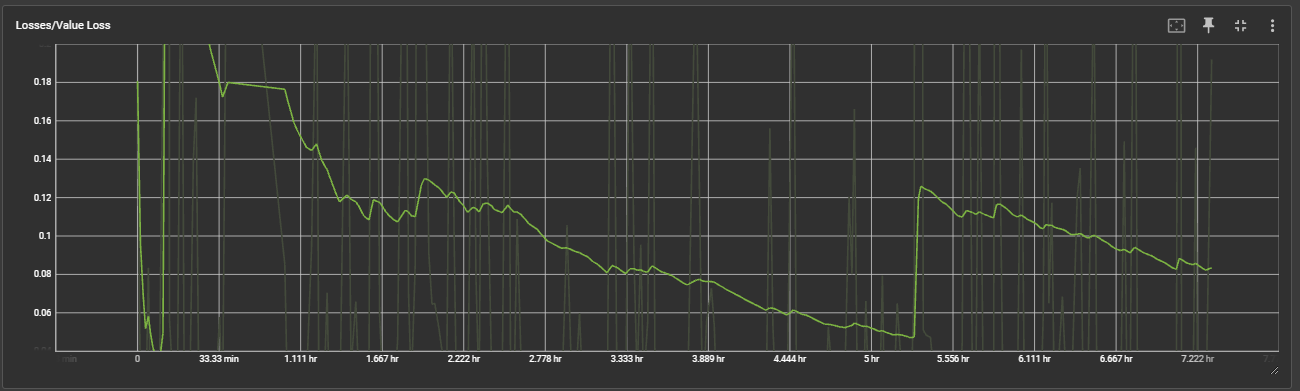
\includegraphics[width=0.8\textwidth]{Figures/App-YokosukaSearchVlueLoss.png}
  \caption{価値関数の平均損失} 
  \label{fig:fig-01}
\end{figure}


\subsection{沼津市の場合}
\begin{figure}[H] 
  \centering 
  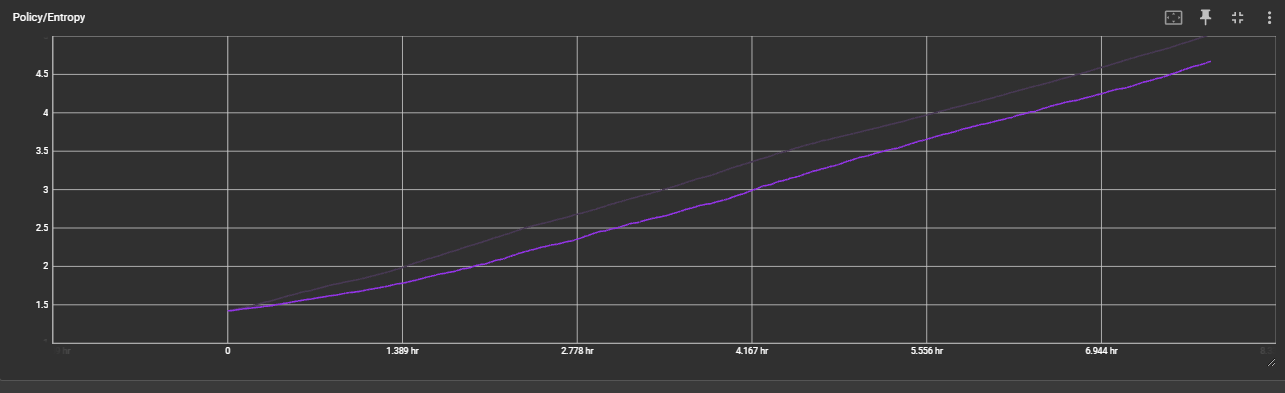
\includegraphics[width=0.8\textwidth]{Figures/NumazuSearch-Entropy.png}
  \caption{エントロピーの推移} 
  \label{fig:fig-01}
\end{figure}
\begin{figure}[H] 
  \centering 
  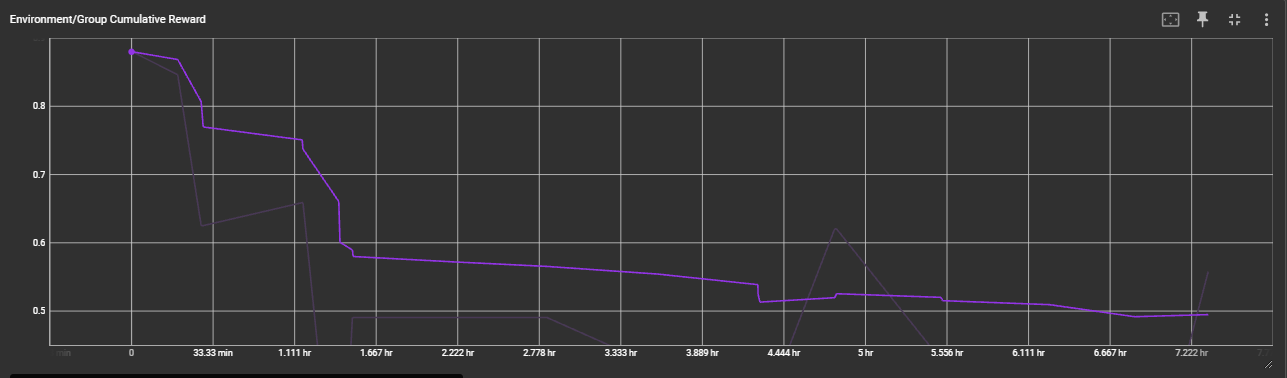
\includegraphics[width=0.8\textwidth]{Figures/NumazuSearch-GroupReward.png}
  \caption{グループ累積報酬の推移} 
  \label{fig:fig-01}
\end{figure}
\begin{figure}[H] 
  \centering 
  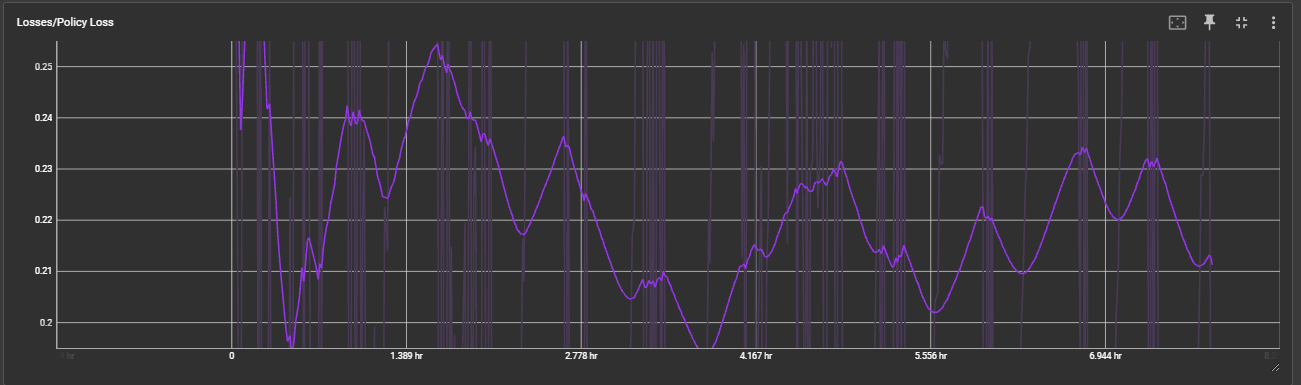
\includegraphics[width=0.8\textwidth]{Figures/NumazuSearch-PolicyLoss.png}
  \caption{ポリシー関数の平均損失} 
  \label{fig:fig-01}
\end{figure}
\begin{figure}[H] 
  \centering 
  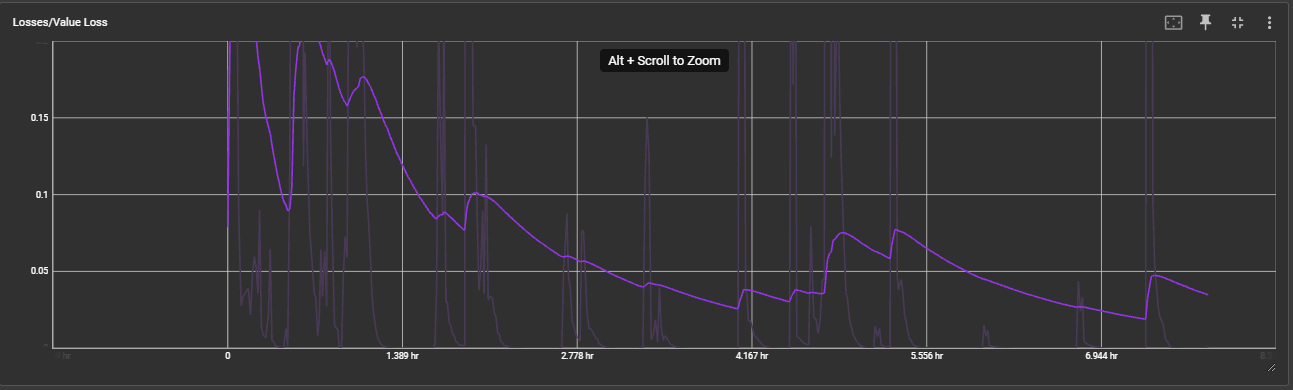
\includegraphics[width=0.8\textwidth]{Figures/NumazuSearch-ValueLoss.png}
  \caption{価値関数の平均損失} 
  \label{fig:fig-01}
\end{figure}

\section{誘導タスクマルチエージェントモデルの学習結果}

\subsection{横須賀市の場合}
\begin{figure}[H] 
  \centering 
  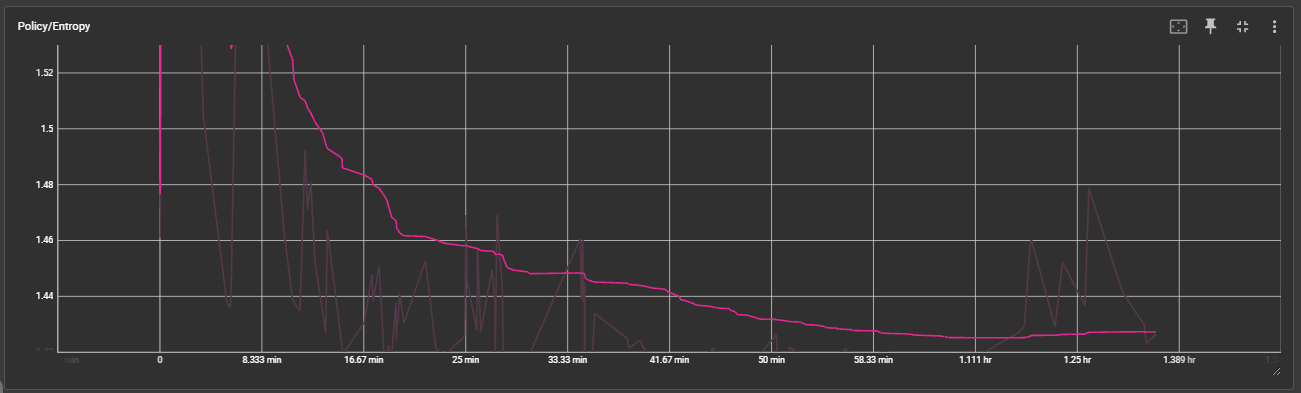
\includegraphics[width=0.8\textwidth]{Figures/Yokosuka-Entropy.png}
  \caption{エントロピーの推移} 
  \label{fig:fig-01}
\end{figure}
\begin{figure}[H] 
  \centering 
  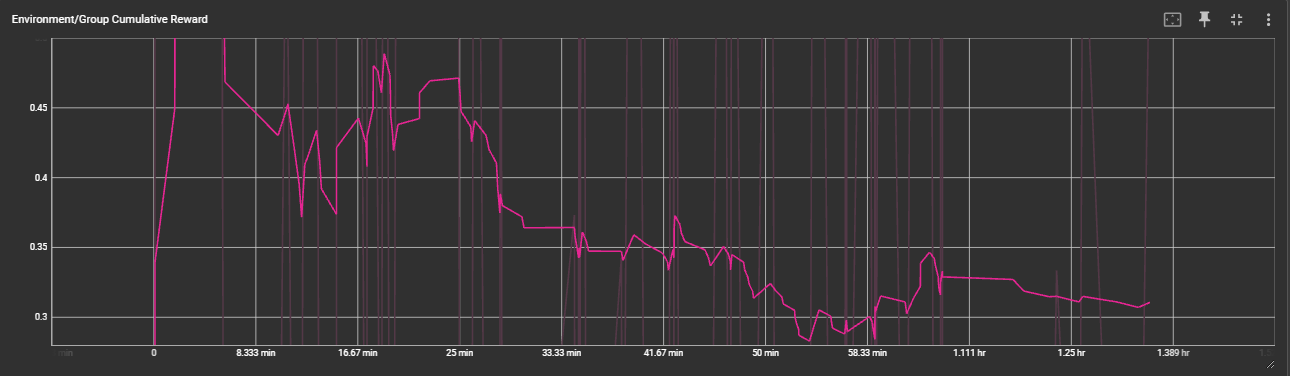
\includegraphics[width=0.8\textwidth]{Figures/Yokosuka-GroupReward.png}
  \caption{グループ累積報酬の推移} 
  \label{fig:fig-01}
\end{figure}
\begin{figure}[H] 
  \centering 
  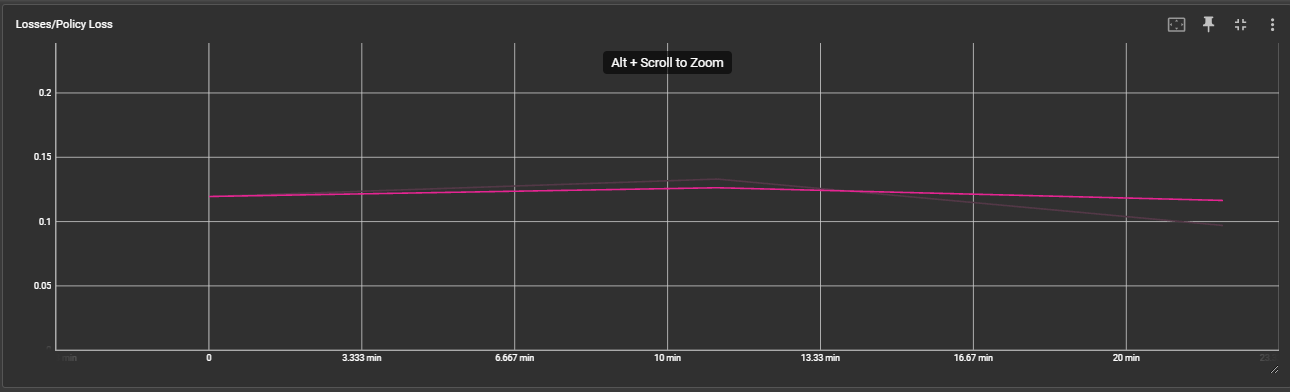
\includegraphics[width=0.8\textwidth]{Figures/Yokosuka-PolycyLoss.png}
  \caption{ポリシー関数の平均損失} 
  \label{fig:fig-01}
\end{figure}
\begin{figure}[H] 
  \centering 
  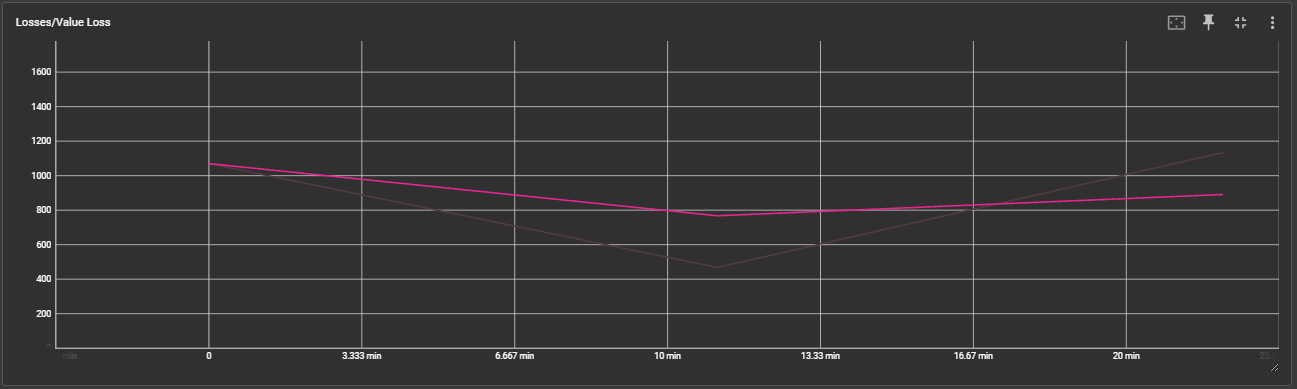
\includegraphics[width=0.8\textwidth]{Figures/YokosukaValueLoss.png}
  \caption{価値関数の平均損失} 
  \label{fig:fig-01}
\end{figure}


\subsection{沼津市の場合}
\begin{figure}[H] 
  \centering 
  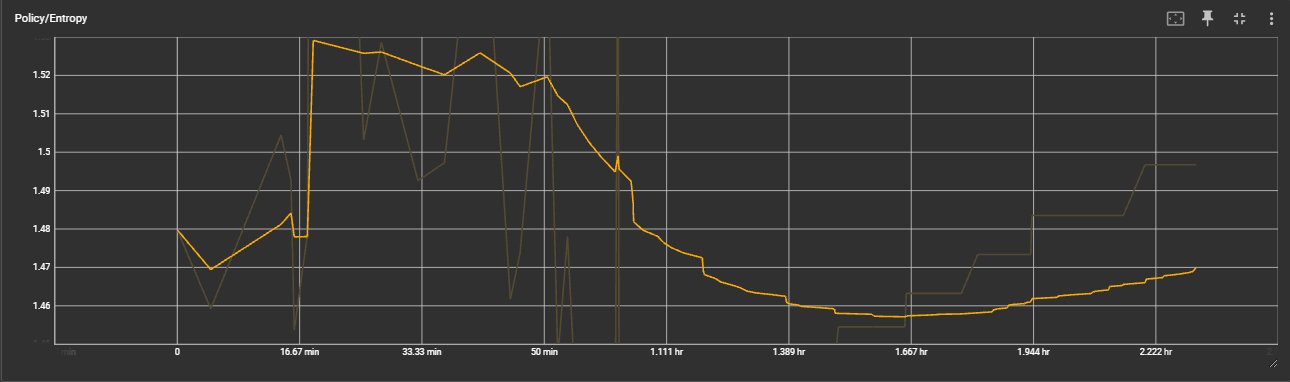
\includegraphics[width=0.8\textwidth]{Figures/NumazuEntropy.png}
  \caption{エントロピーの推移} 
  \label{fig:fig-01}
\end{figure}
\begin{figure}[H] 
  \centering 
  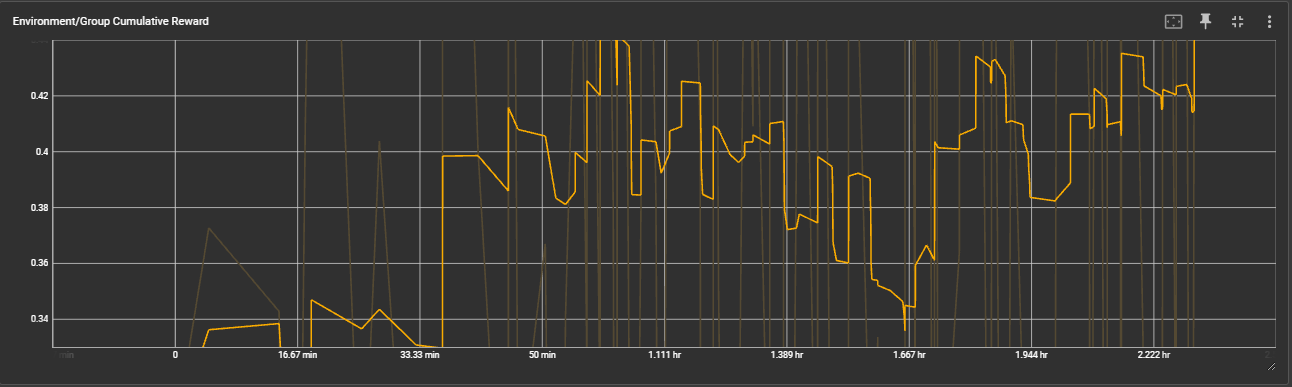
\includegraphics[width=0.8\textwidth]{Figures/NumazuGroupReward.png}
  \caption{グループ累積報酬の推移} 
  \label{fig:fig-01}
\end{figure}
\begin{figure}[H] 
  \centering 
  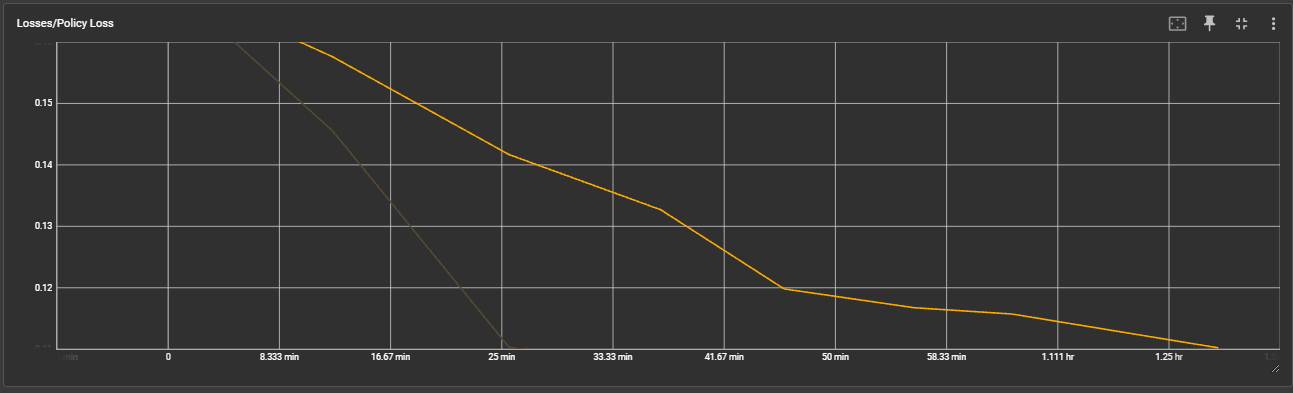
\includegraphics[width=0.8\textwidth]{Figures/NumazuPolicyLoss.png}
  \caption{ポリシー関数の平均損失} 
  \label{fig:fig-01}
\end{figure}
\begin{figure}[H] 
  \centering 
  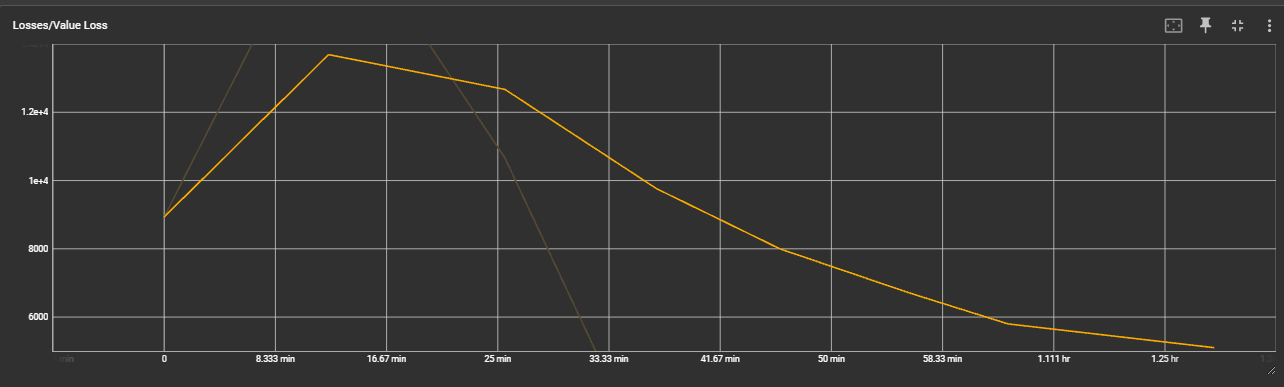
\includegraphics[width=0.8\textwidth]{Figures/NumazuValueLoss.png}
  \caption{価値関数の平均損失} 
  \label{fig:fig-01}
\end{figure}

\section{探索タスクにおける発見率の推移}

\subsection{横須賀市の場合}
\begin{figure}[H] 
  \centering 
  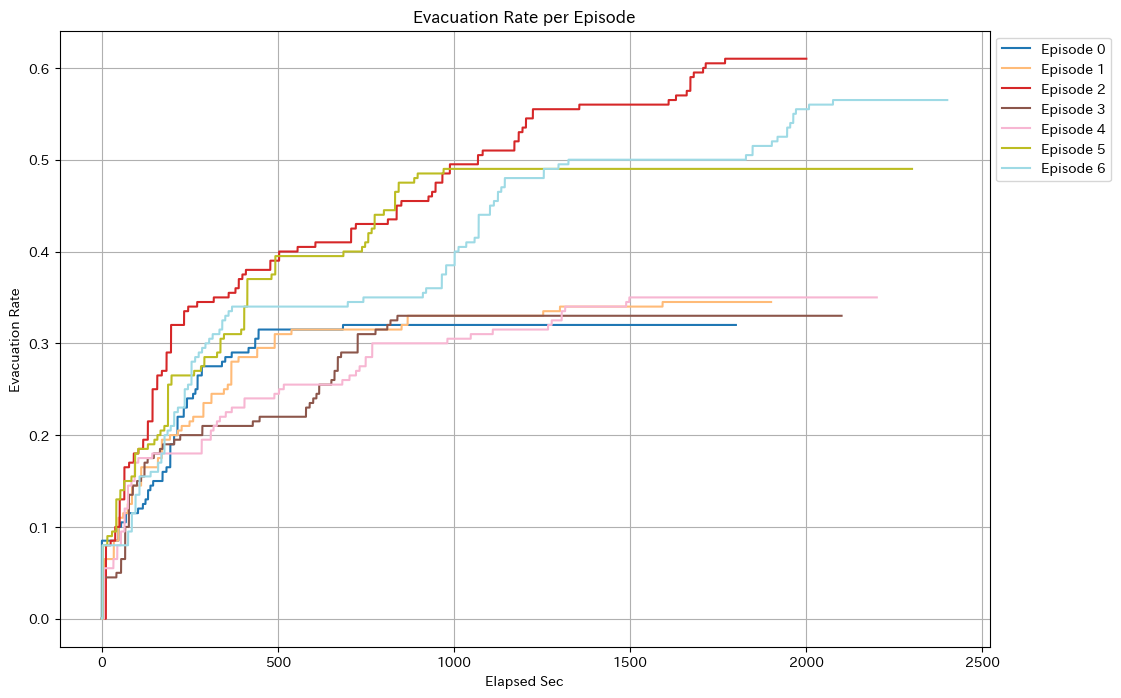
\includegraphics[width=0.8\textwidth]{Figures/YokosukaSearch-RuleResult.png}
  \caption{ルールベースでの発見率の推移} 
\end{figure}

\begin{figure}[H] 
  \centering 
  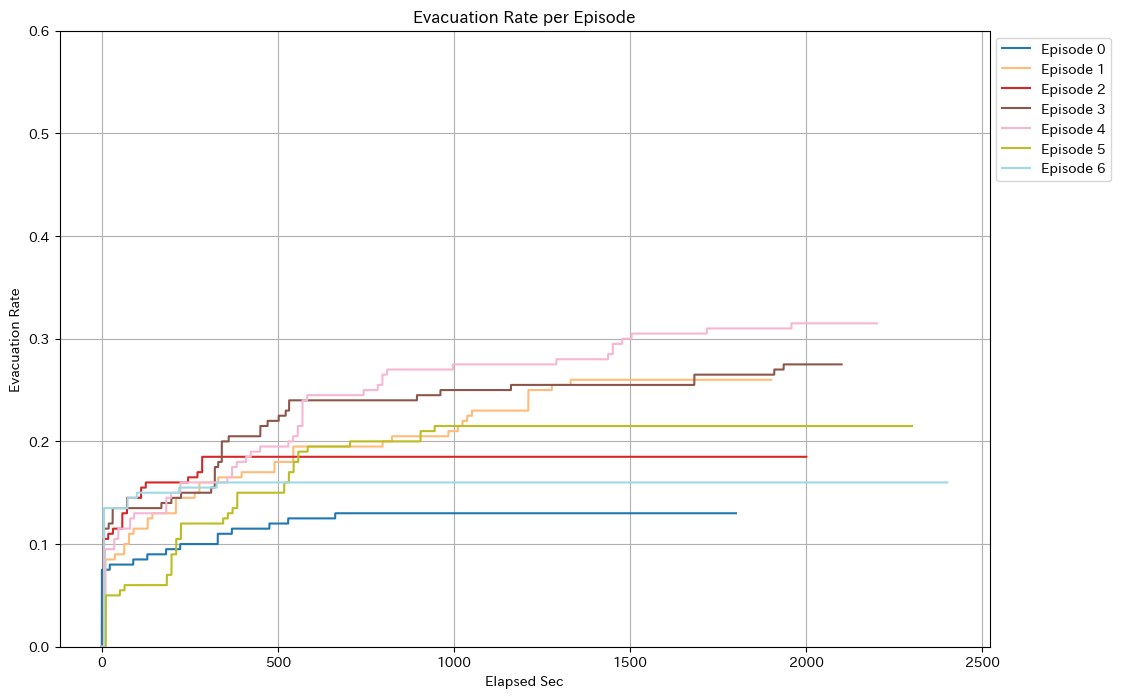
\includegraphics[width=0.8\textwidth]{Figures/YokosukaSearch-AgentsResult.png}
  \caption{マルチエージェントモデルでの発見率の推移} 
\end{figure}

\subsection{沼津市の場合}
\begin{figure}[H] 
  \centering 
  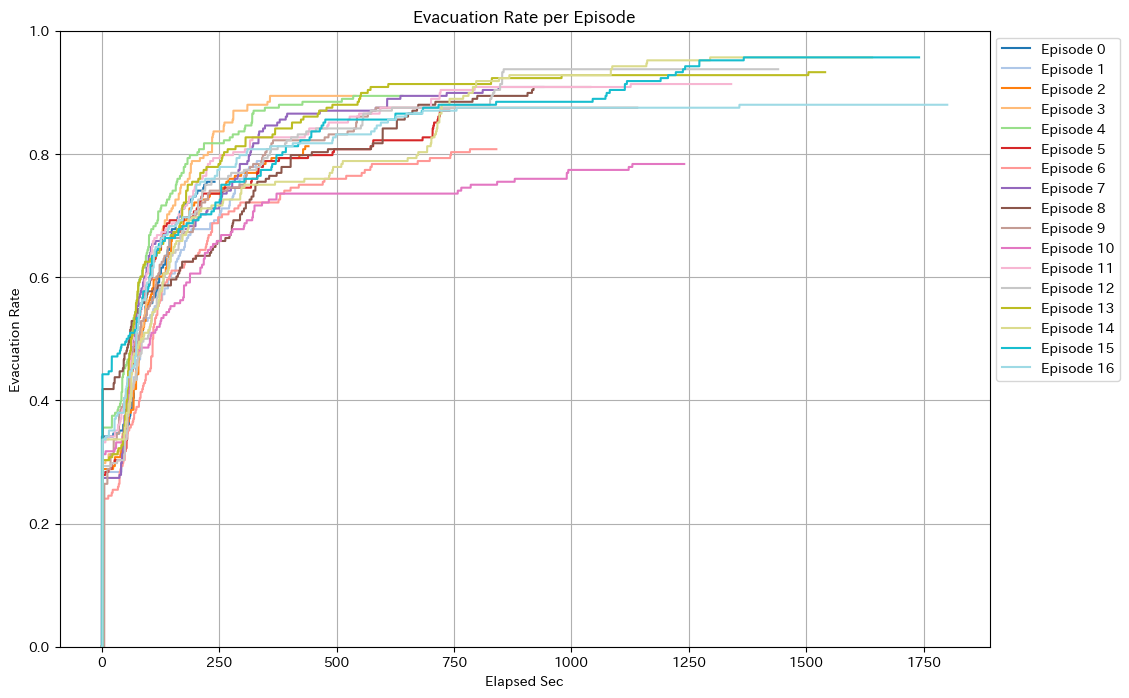
\includegraphics[width=0.8\textwidth]{Figures/NumazuSearch-RuleResult.png}
  \caption{ルールベースでの発見率の推移}
\end{figure}

\begin{figure}[H] 
  \centering 
  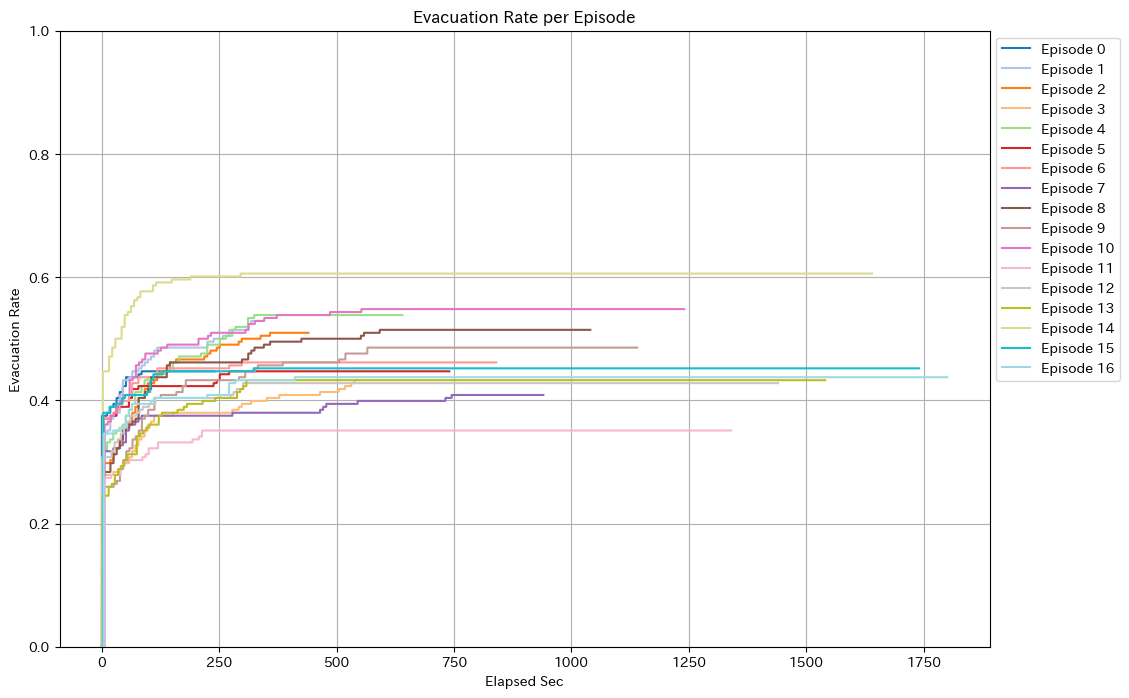
\includegraphics[width=0.8\textwidth]{Figures/NumazuSearch-AgentsResult.png}
  \caption{マルチエージェントモデルでの発見率の推移}
\end{figure}

\section{誘導タスクにおける避難完了率の推移}

\subsection{横須賀市の場合}

\begin{figure}[H]
  \centering
  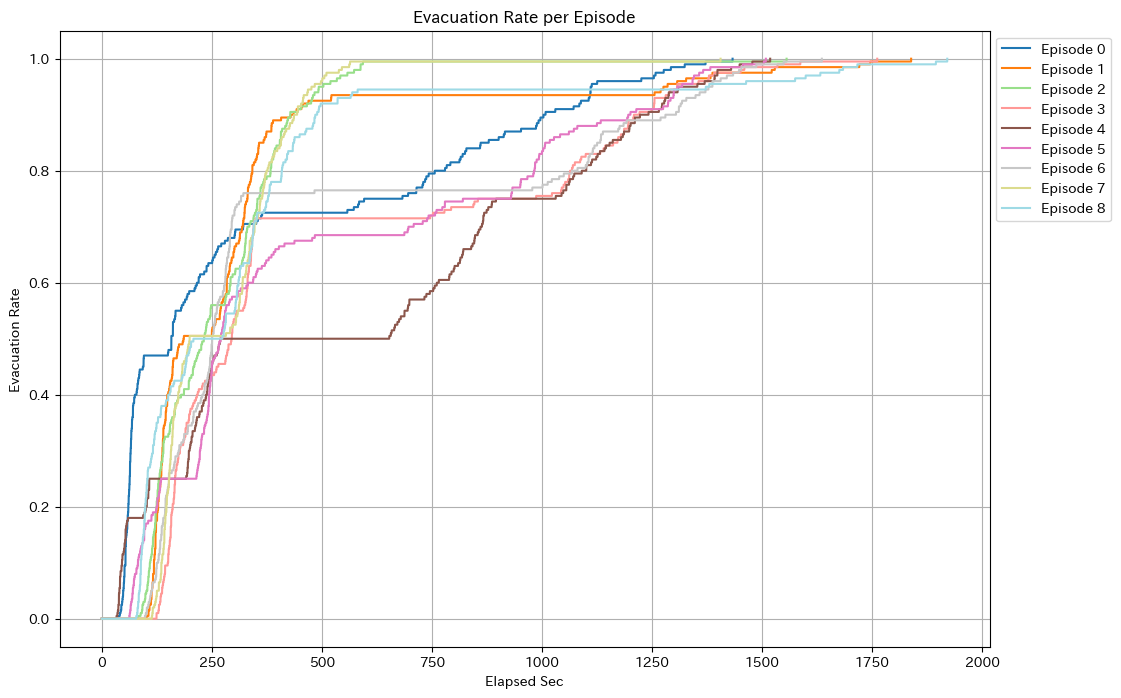
\includegraphics[width=0.8\textwidth]{Figures/Yokosuka-EvaOnly-ERE.png}
  \caption{避難者のみ(誘導無)での避難完了率の推移}
\end{figure}

\begin{figure}[H] 
  \centering 
  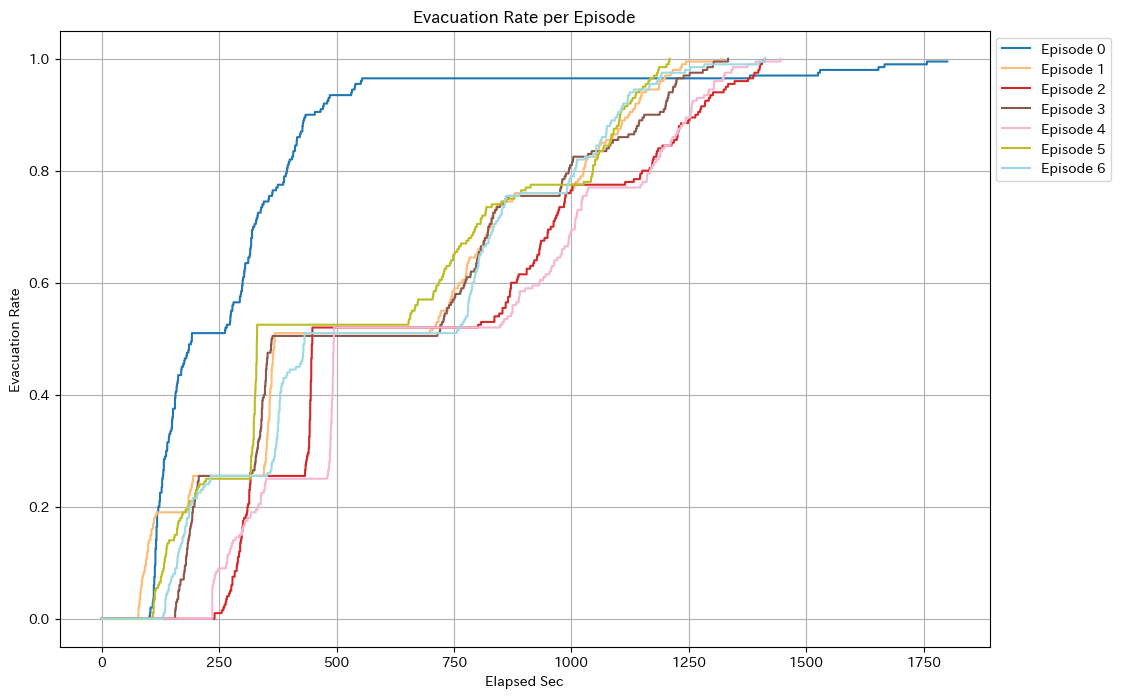
\includegraphics[width=0.8\textwidth]{Figures/Yokosuka-RuleModel-ERE.png}
  \caption{ルールベースでの避難完了率の推移}
\end{figure}

\begin{figure}[H] 
  \centering 
  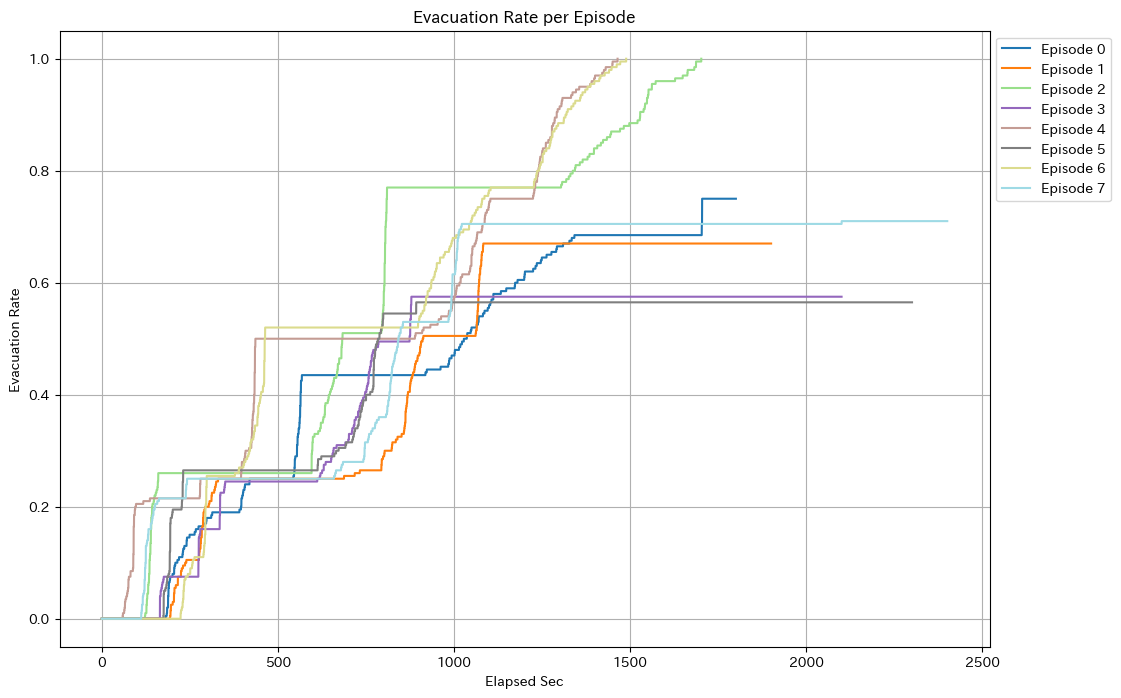
\includegraphics[width=0.8\textwidth]{Figures/Yokosuka-AgentModel-ERE.png}
  \caption{マルチエージェントモデルでの避難完了率の推移}
\end{figure}

\subsection{沼津市の場合}

\begin{figure}[H]
  \centering
  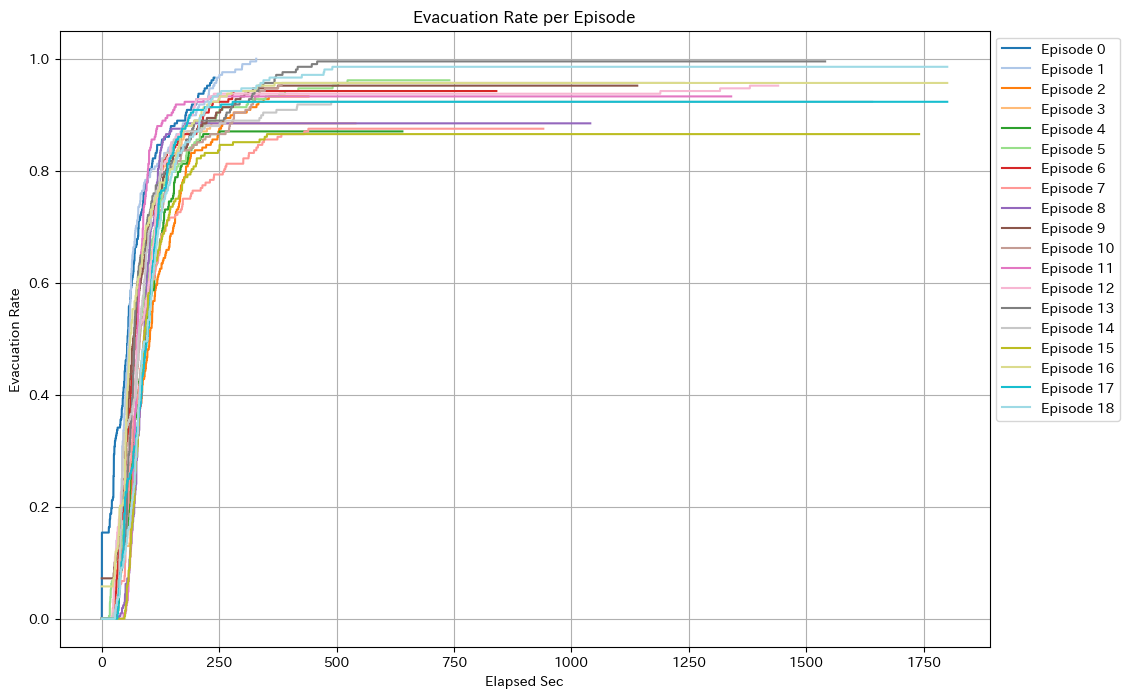
\includegraphics[width=0.8\textwidth]{Figures/Numazu-EvaOnly-ERE.png}
  \caption{避難者のみ(誘導無)での避難完了率の推移}
\end{figure}

\begin{figure}[H] 
  \centering 
  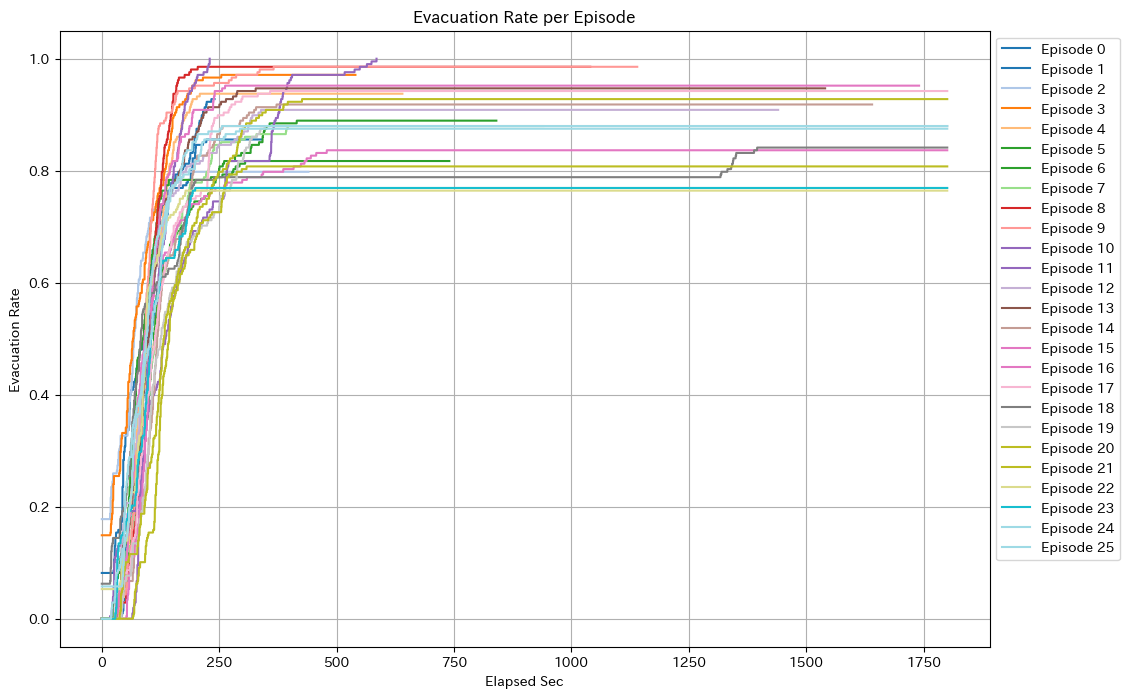
\includegraphics[width=0.8\textwidth]{Figures/Numazu-RuleModel-ERE.png}
  \caption{ルールベースでの避難完了率の推移}

\end{figure}

\begin{figure}[H] 
  \centering 
  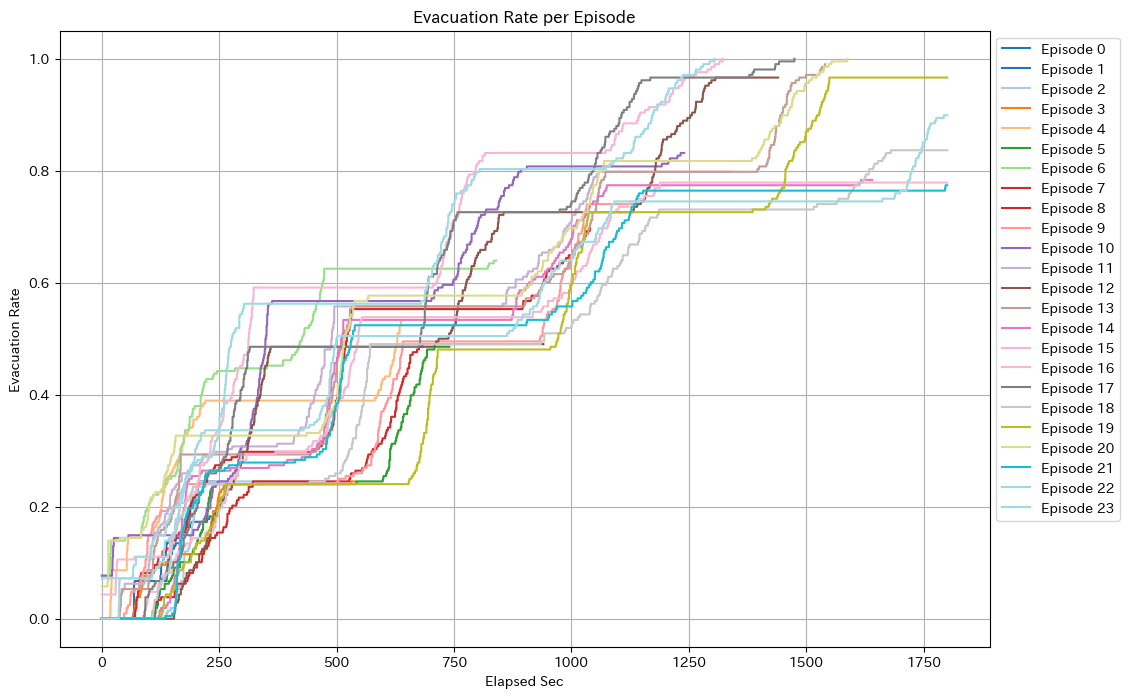
\includegraphics[width=0.8\textwidth]{Figures/Numazu-AgentModel-ERE.png}
  \caption{マルチエージェントモデルでの避難完了率の推移}
\end{figure}


